\begin{frame}{}{}
 
We define and explore in simulation several (meta)rules for the local
evolution of generative rules for 1D and 2D {\fontspec{Bookhands}
  cellular\hspace{.5em}automata}.  Our implementation uses strategies
from conceptual blending.  We discuss potential applications to
modelling social dynamics.
\end{frame}

\part{Background}
\frame{\partpage}

\begin{frame}{Cellular Automata}{}\label{intro-to-ca}
Each elementary 1-dimensional cellular automaton (1D CA) corresponds to a mapping from all eight \emph{triples} formed of
0's and 1's to the set \{0,1\}.
Thus, for example the rule $\mathbf{01010100}$
is defined as the following operation:
\bigskip

\begin{tabular}{l@{\hskip -.07in}p{2.5in}}
\begin{fminipage}{1.6in}
\lstinputlisting{exampleca.tex}
\end{fminipage} &
\raisebox{.2in}{\begin{minipage}{2.5in}
The rules determine the next generation of a 1D CA locally, where each cell inherits from three ``parents''.

\medskip

In the example,
\boxed{0\mystrut}\boxed{0\mystrut}\boxed{0\mystrut} $\mapsto$
\boxed{0\mystrut} and
\boxed{0\mystrut}\boxed{0\mystrut}\boxed{1\mystrut} $\mapsto$
\boxed{1\mystrut} and so on.
\end{minipage}}
\end{tabular}
\end{frame}

\begin{frame}{Cellular Automata, ctd.}{}
%% These rules can then be used to fill in a 2-dimensional grid, by
%% starting by creating a row of cells with fixed values at the top, and
%% defining a suitable condition on the edges, for example, saying they
%% are always \boxed{0\mystrut}.  We usually depict \boxed{0\mystrut} as
%% \framebox(8,8){} and \boxed{1\mystrut} as $\blacksquare$.
\emph{It is a remarkable fact that some of these systems are} {\fontspec{Bookhands}Turing\bsp complete}.\vspace{.2in}

\pause
\begin{center}
\begin{minipage}{.97\textwidth}
{\centering
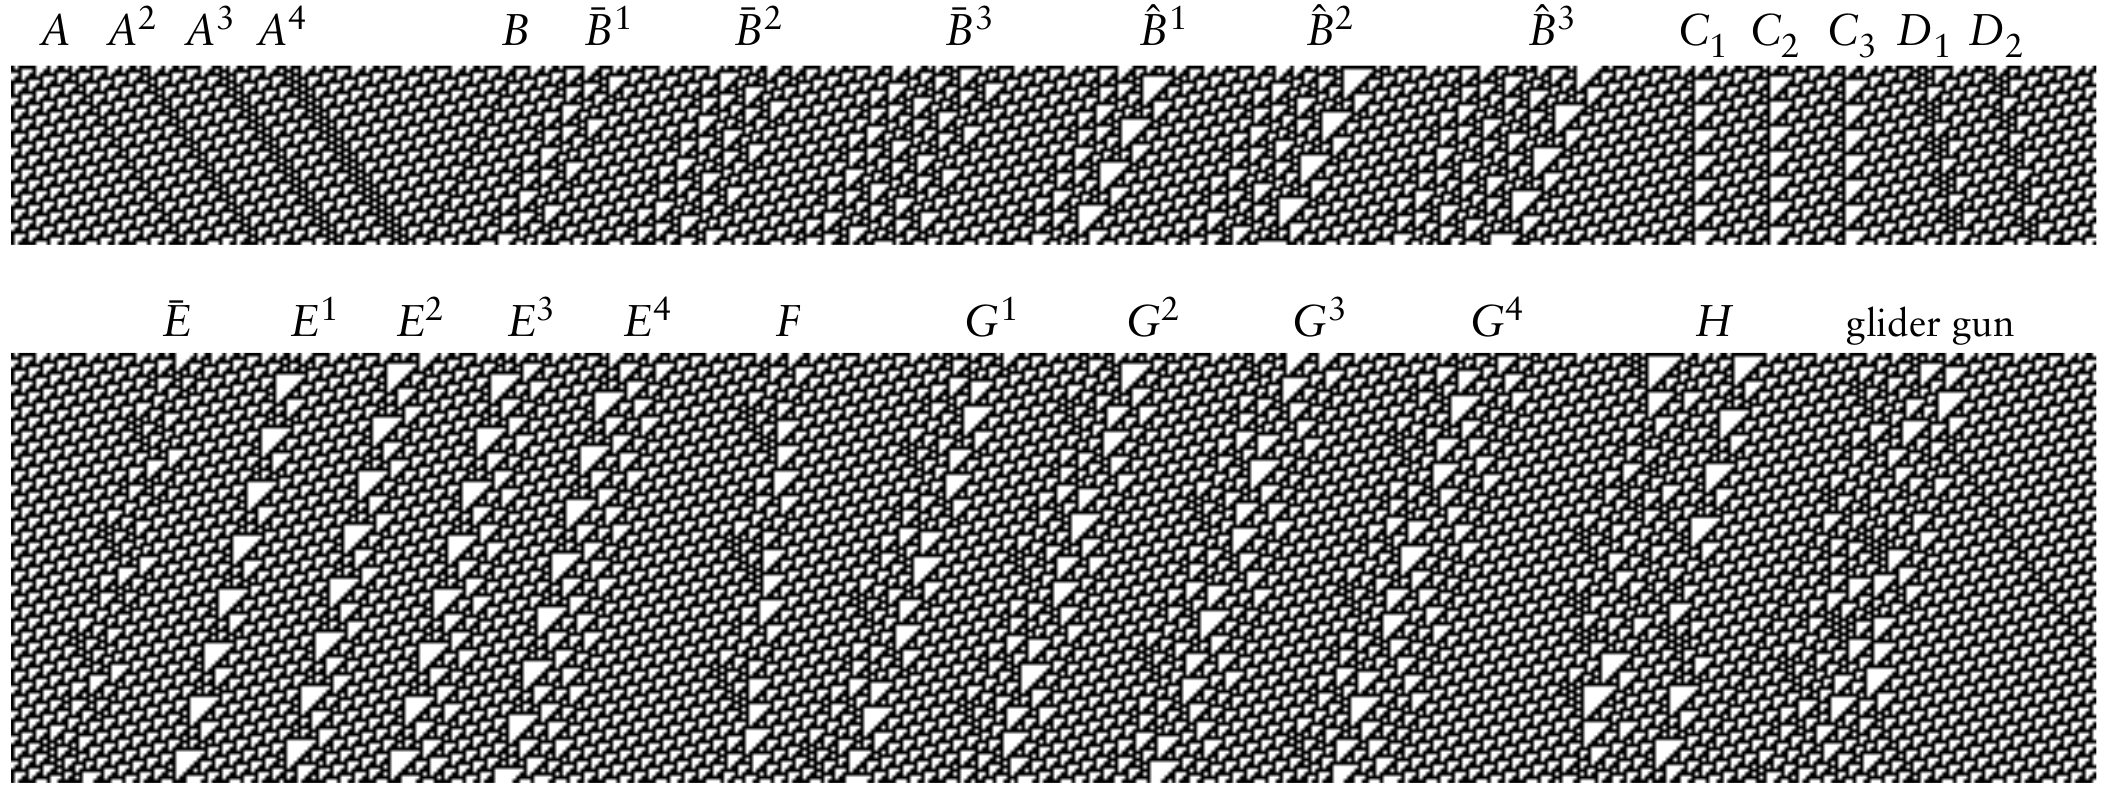
\includegraphics[width=.95\textwidth]{cook}

M. Cook, Universality in elementary cellular automata, \emph{Complex Systems}, 15 (2004) 1–40

\par}
\end{minipage}
\end{center}
\end{frame}

\part{MetaCAs}
\frame{\partpage}

\begin{frame}{Evolving genotypes}{}
A {\fontspec{Bookhands}MetaCA } evolves a cellular automaton with \emph{{\color{red}2}{\color{LimeGreen}5}{\color{blue}6}} ($=2^8$) possible
states -- rather than the traditional 2, \framebox(8,8){} and $\blacksquare$.
Each state of a MetaCA cell corresponds to a ``1D CA rule.''  For example:\\[.3in]
\begin{tabular}{l@{\hskip -.1in}p{2.5in}}
\begin{fminipage}{1.7in}
\lstinputlisting{example-metaca.tex}
\end{fminipage} & 
\vspace*{-.7in}
$01101110\times \mathbf{01010100}\times 01010101$: Apply the central rule ``allele-wise'', i.e.~look up each row of triples on the left in the table
from Slide \ref{intro-to-ca}. 
\end{tabular}
\end{frame}

\begin{frame}{Initial experiment}{(not particularly impressive)}
\begin{center}
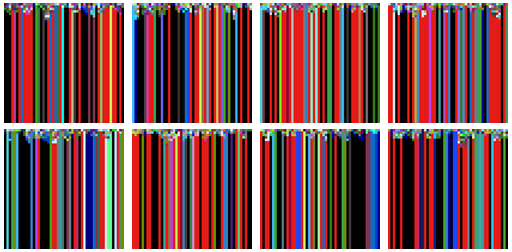
\includegraphics[width=.9\textwidth]{paint-drips2.png}

\pause
paint-drips2.png
\end{center}
\end{frame}

\begin{frame}{Introducing blending dynamics}{}
We realised we could apply a more ``COINVENTish'' rule to build
``blending'' into the multiplication.  If the two neighbours are the
same, simply use their common value as the final result, otherwise apply
the local rule to that allele, as above.
\begin{center}
\begin{fminipage}{2.7in}
\lstinputlisting{example-blending-metaca.tex}
\end{fminipage} 

$01101110\times_b \mathbf{01010100}\times_b 01010101$ 
\end{center}
\end{frame}

\begin{frame}[fragile]{Here's some super easy category theory}{}

Here $\mathfrak{g}_{\cdot}$ is a (reverse) generalisation from an input space to the \emph{generic space}, and $\mathfrak{p}_{\cdot}$ a (reverse) \emph{projection} from the colimit.

\begin{columns}[]
\begin{column}[T]{5.5cm}
\begin{tikzcd}
     &                  \{0\}   &   & \\
\{0\} \arrow[ru,swap,"\mathfrak{p}_1"]&             & \{0\} \arrow[lu,"\mathfrak{p}_2"]&     \\
     &              \{0\} \arrow[lu,swap,"\mathfrak{g}_1"] \arrow[ru,"\mathfrak{g}_2"] \arrow[uu,dashed]       &   &               
\end{tikzcd}
\vspace*{.2cm}

{\centering {\small All structure is shared; the ``blend'' is the only thing it could be.}\par}
\end{column}
\begin{column}[T]{5.5cm}
\begin{tikzcd}
     &                  \{0,1\}   &   & \\
\{0\} \arrow[ru,swap,"\mathfrak{p}_1"]&             & \{1\} \arrow[lu,"\mathfrak{p}_2"]&     \\
     &              \{\} \arrow[lu,swap,"\mathfrak{g}_1"] \arrow[ru,"\mathfrak{g}_2"] \arrow[uu,dashed]       &   &               
\end{tikzcd}
\vspace*{.2cm}

{\centering {\small \emph{No} structure is shared; we need \emph{some} way to ``refine'' the blend to produce something useful.  Luckily we have one\ldots}\par}
\end{column}
\end{columns}
\end{frame}

\begin{frame}{Second experiment}{}
\begin{center}
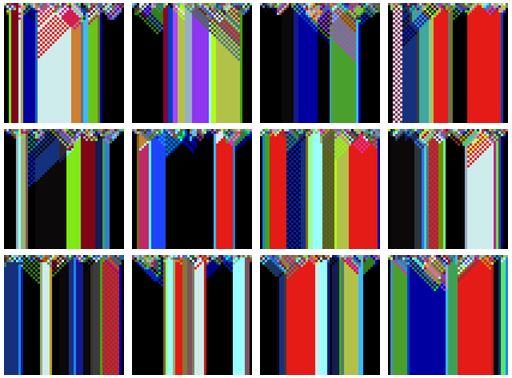
\includegraphics[width=.9\textwidth]{metaca2.png}
\pause

wow, blending really works!
\end{center}
\end{frame}

\part{More 1D experiments}
\frame{\partpage}

\begin{frame}{Phenotype determined by the genotype}{}
Apply the local genotype rule $g\in 2^8$ from the left to the corresponding phenotype data \boxed{a\mystrut}\boxed{b\mystrut}\boxed{c\mystrut} on the right to compute the next value for the phenotype.
\begin{center}

\includegraphics[width=.9\textwidth]{genotype-determines-phenotype.png}
\pause

OK, maybe blending doesn't solve all our problems
\end{center}
\end{frame}

\begin{frame}{Adding mutation}{}
\begin{center}
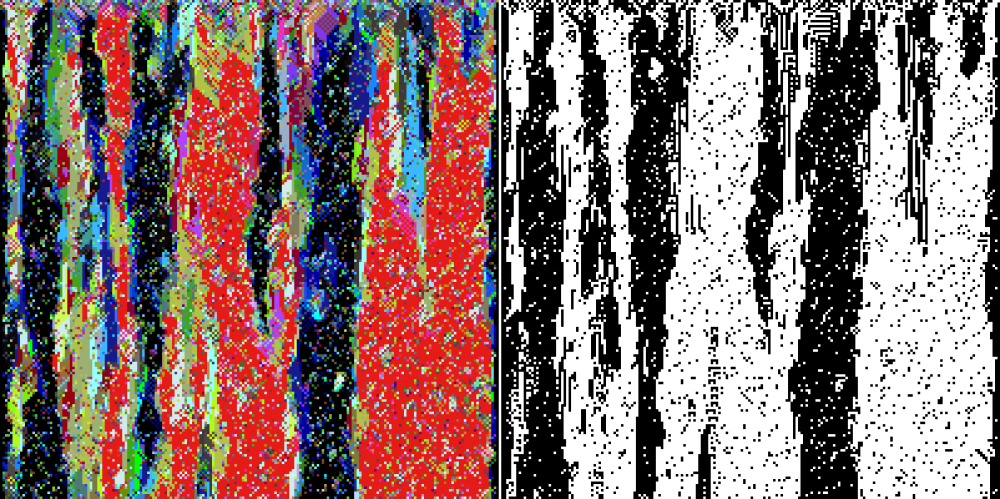
\includegraphics[width=.9\textwidth]{lamp-down-low.png}
\end{center}
\end{frame}

\begin{frame}{A skewed mutation rule}{Hurrah for human error!}
\begin{center}
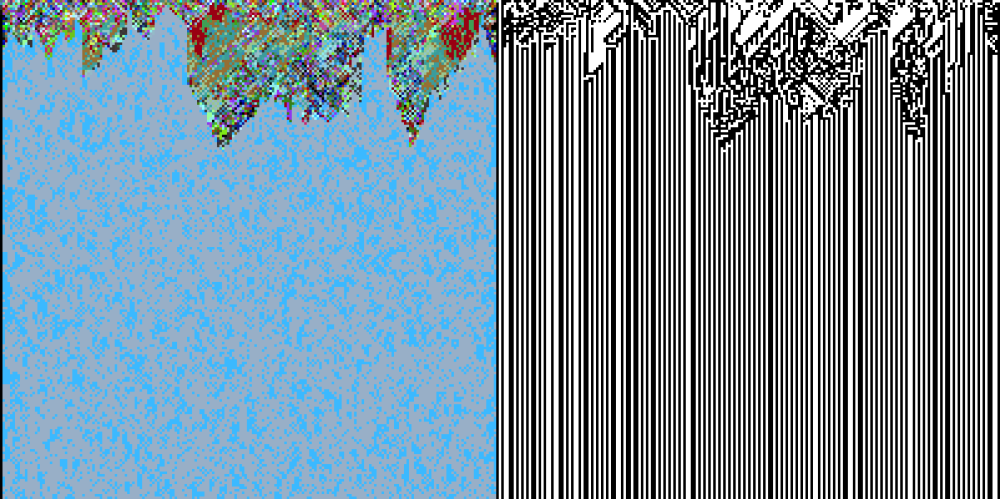
\includegraphics[width=.9\textwidth]{reef.png}
\end{center}
\end{frame}

\begin{frame}[fragile]{A possible critique of basic blending}{}
Straightforward blending is actually just a censored version of Wolfram's Rule 23.  So, no matter what ``local rule'' we use, a lot of the results are pre-determined, as a blend of the local rule and Rule 23.  Can we get more flexibility?
\begin{columns}
\begin{column}[T]{.2in}
\end{column}
%

\begin{column}[T]{1.6in}
\begin{fminipage}{1.6in}
\lstinputlisting{rule23.tex}
\end{fminipage}
\end{column}

% 
\begin{column}[T]{2in}
\begin{fminipage}{1.6in}
\lstinputlisting{censored-rule23.tex}
\end{fminipage}
\end{column}

%
\begin{column}[T]{.05in}
\end{column}
%
\end{columns}

\end{frame}

\begin{frame}{How about a more flexible ``template''?}{Introducing an epigenetic (``Baldwin'') effect}
The standard template could be understood to be generated by locking in
%
\boxed{0\mystrut}\boxed{0\mystrut}\boxed{0\mystrut} $\mapsto$ \boxed{0\mystrut}
%
along with a ``variation''
%%
\boxed{0\mystrut}\boxed{1\mystrut}\boxed{0\mystrut} $\mapsto$
\boxed{0\mystrut} and the bitwise complements of these.  A wider class of
templates could be calculated from arbitrary phenotype data by the same
operations. 

\medskip

The observed phenotype data
\boxed{a\mystrut}\boxed{b\mystrut}\boxed{c\mystrut} $\mapsto$ \boxed{d\mystrut}
would then be ``locked in'' at the genotype level as a template in the next round of evolution, along with:

\smallskip
{\centering
\boxed{a\mystrut}\boxed{b^\prime\mystrut}\boxed{c\mystrut} $\mapsto$ \boxed{d\mystrut},\quad
\boxed{a^\prime\mystrut}\boxed{b^\prime\mystrut}\boxed{c^\prime\mystrut} $\mapsto$ \boxed{d^\prime\mystrut}\quad
and\quad
\boxed{a^\prime\mystrut}\boxed{b\mystrut}\boxed{c^\prime\mystrut} $\mapsto$ \boxed{d^\prime\mystrut}, \par}
\smallskip

where prime denotes bit-complement.
\end{frame}

\begin{frame}{New!}{}
\begin{center}
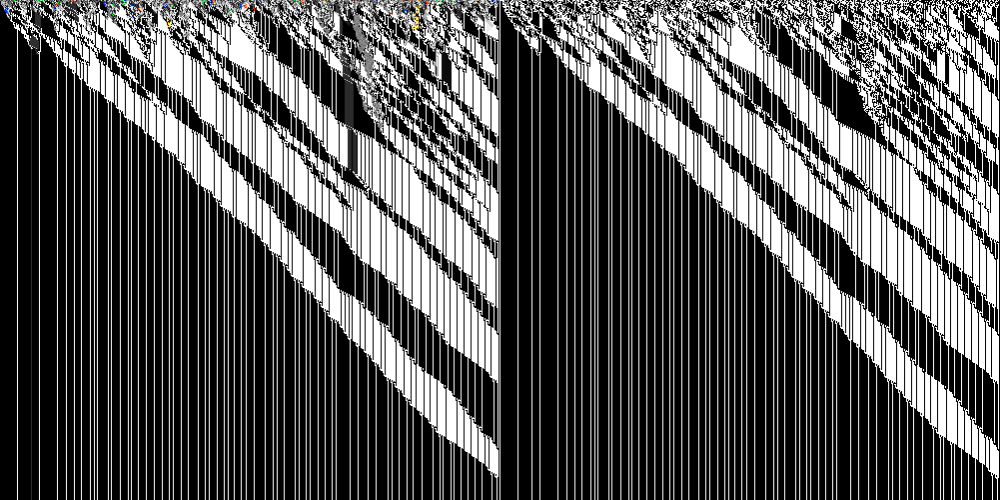
\includegraphics[width=.9\textwidth]{drift2.png}
\pause

100\% deterministic after initial random seeding\\
\pause
But lots of Rule 0 (00000000) and Rule 256 (11111111)
\end{center}
\end{frame}

\begin{frame}{Adding mutation again}{}
\begin{center}
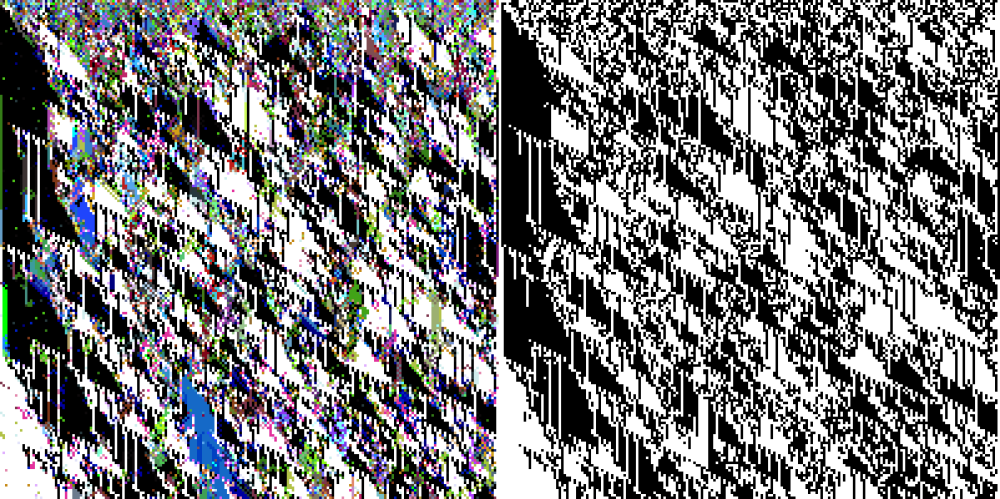
\includegraphics[width=.9\textwidth]{slight-randomness.png}
\pause

Still lots of Rule 0 and Rule 256
\end{center}
\end{frame}

\begin{frame}{With a more ``selective'' mutation}{}
\begin{center}
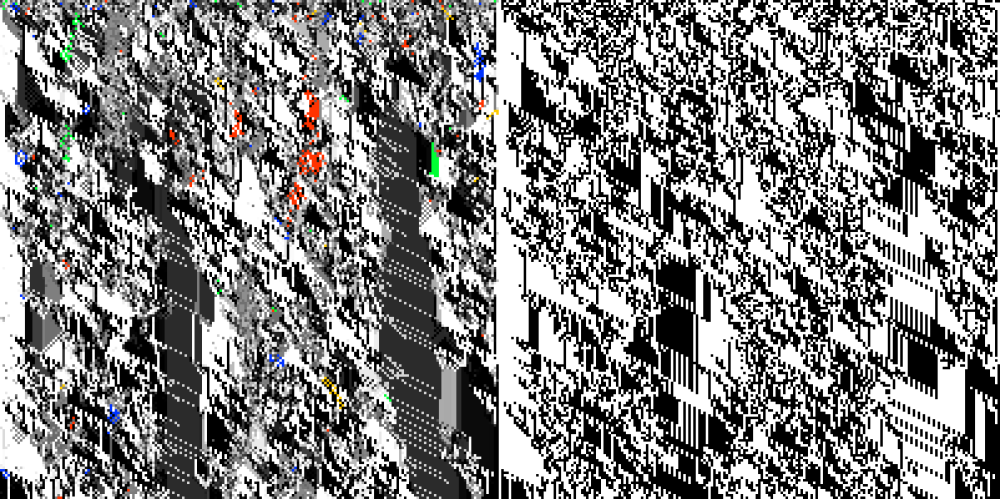
\includegraphics[width=.9\textwidth]{populations.png}
\pause

Intuition: the number of 0's and 1's in the genotype should be approximately equal
\end{center}
\end{frame}

\part{2D experiments}
\frame{\partpage}

\begin{frame}{}{}
\vspace*{-1cm}
\begin{center}
\item{Conway's {\fontspec{Bookhands}Game\bsp of\bsp Life} rule:}\vspace*{.1cm}
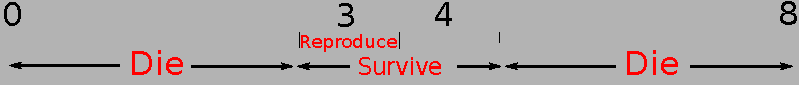
\includegraphics[width=.9\textwidth]{conway.pdf}
\item{
\begin{fminipage}{7cm}
\begin{tabular}{cc}
\# alive neighbours & new state\\
3  & alive\\
4  & same\\
>4 & dead\\
<3 & dead\\
\end{tabular}
\end{fminipage}
}
\item{Generalised (local) rule (i.e.~``genotype''):}\vspace*{.1cm}
  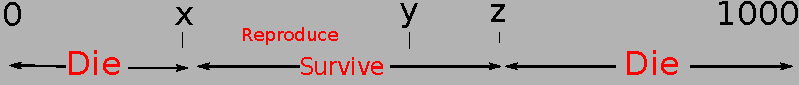
\includegraphics[width=.9\textwidth]{2dgenotype.pdf}
\begin{fminipage}{8.2cm}
$x\leq\sum \textit{weight\ of\ neighbours}<y\Rightarrow\textit{alive}$\newline
$y\leq\sum \textit{weight\ of\ neighbours}<z\Rightarrow\textit{same}$
\end{fminipage}
a cell's $\textit{weight}$ is its ``phenotype''.
\end{center}
\end{frame}

\begin{frame}{Extending blending to 2D CAs}{Example: \emph{union blend} selects largest ``reproduce'' window}
\begin{center}
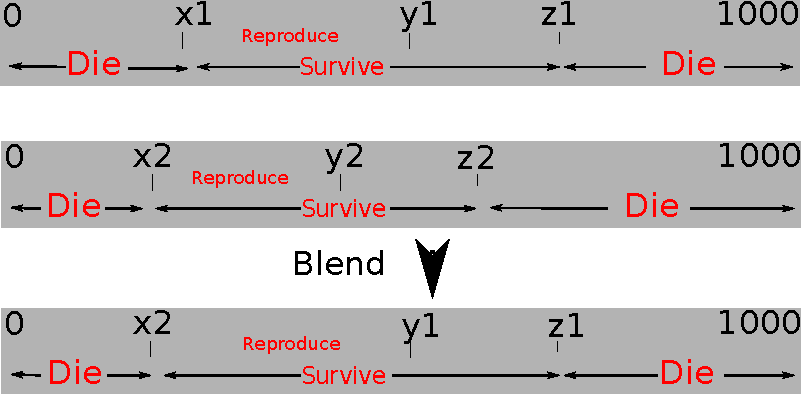
\includegraphics[width=.9\textwidth]{2dgenotypeblend.pdf}
\end{center}
\end{frame}

\begin{frame}{Results}{}
{\footnotesize ``Compute the union blend for any living cell, and all neighbours; new weight is average of living neighbours, including self.''}
\begin{center}
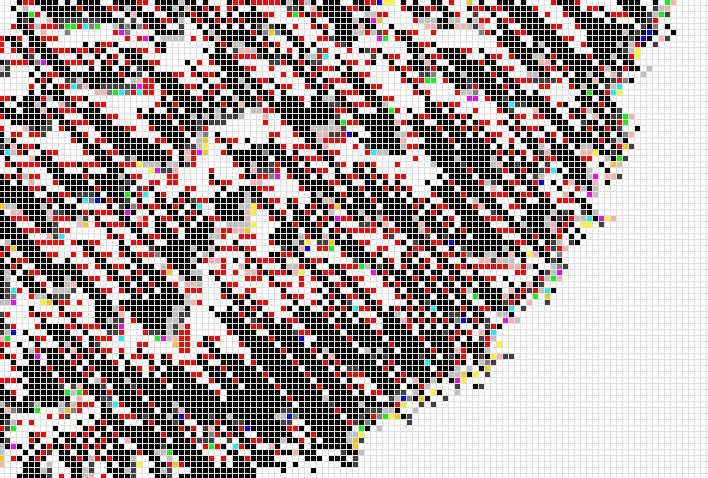
\includegraphics[width=.9\textwidth]{300002d.jpg}
\end{center}
\end{frame}

\part{Discussion}
\frame{\partpage}

\begin{frame}{An extended view on the social}{Social $\Leftrightarrow$ Emergent}
{\small ``The social nature of the present arises out of its emergence.''
% \emph{The philosophy of the present}
%% I
   %% am referring to the process of readjustment that emergence
   %% involves. Nature takes on new characters, for example with the
   %% appearance of life, or the stellar system takes on new characters
   %% with the loss of mass by the collapse of atoms through the
   %% processes that go on within a star. There is an adjustment to this
   %% new situation. The new objects enter into relationship with the
   %% old. The determining conditions of passage set the conditions under
   %% which they survive, and the old objects enter into new relations
   %% with what has arisen. I am here using the term ``social'' with
   %% reference not to the new system, but to the process of
   %% readjustment.

\medskip

% [O]bjects are constituted in terms of meanings within the social process of experience and behavior through the mutual adjustment to one another of the responses or actions of the various individual organisms involved in that process, an adjustment made possible by means of a communication which takes the form of a conversation of gestures in the earlier evolutionary stages of that process, and of language in its later stages.

% [A] gesture is a symbol of the result of the given social act of one organism (the organism making it) in so far as it is responded to by another organism (thereby also involved in that act) as indicating that result.

``Symbolization constitutes objects not constituted before, objects which would not exist except for the context of social relationships wherein symbolization occurs.''
 % \emph{Mind, Self, and Society}
} \qquad\qquad \raisebox{-.2cm}{\fontspec{Bookhands}George\bsp H.\bsp Mead}
\end{frame}

\begin{frame}{An ethical view on blending}{Blending as a blend?}
\begin{columns}[onlytextwidth]
\begin{column}[T]{3in}
{\fontspec{Bookhands}Carol\bsp Gilligan} describes an
\emph{ethic of care} that seeks to defend the
relationships that obtain in a given situation.  In blending this is
manifested by the question ``Have my neighbours already formed a
consensus?''  Blending extends the local rule, which would correspond
to Lawrence Kohlberg's \emph{ethic of justice}.
\end{column}
\begin{column}[T]{.1in}
\end{column}
%\pause
\begin{column}[T]{2in}
\vspace*{.2in}
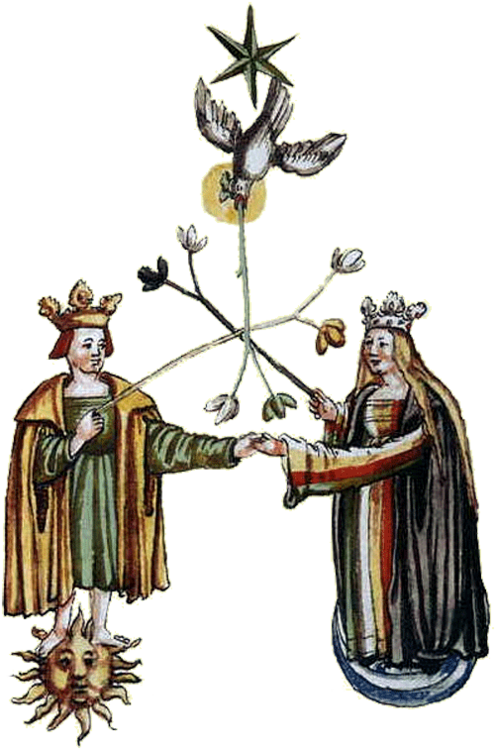
\includegraphics[width=.7\textwidth]{weddingt}
\end{column}
\end{columns}
\end{frame}

\begin{frame}{A philosophical view on life}{Transfer}
{\small ``Regarded from this point of view, \emph{life is like a current passing from germ to germ through the medium of a developed organism}. It is as if the organism itself were only an excrescence, a bud caused to sprout by the former germ endeavoring to continue itself in a new germ. The essential thing is the \emph{continuous progress} indefinitely pursued, an invisible progress, on which each visible organism rides during the short interval of time given it to live.''} \qquad\qquad \raisebox{-.2cm}{\fontspec{Bookhands}Henri\bsp Bergson}
\end{frame}

\begin{frame}{A philosophical view on life, ctd.}{Growth}
``Chemists have pointed out that even in the organic---not to go so far as the organized---science has reconstructed hitherto nothing but waste products of vital activity; the peculiarly active plastic substances obstinately defy synthesis.  One of the most notable naturalists of our time has insisted on the opposition of two orders of phenomena observed in living tissues, \emph{anagenesis} and \emph{katagenesis}. The r\^{o}le of the anagenetic energies is to raise the inferior energies to their own level by assimilating inorganic substances.''\quad \raisebox{-.2cm}{\fontspec{Bookhands}Bergson}
\end{frame}

\begin{frame}{A philosophical view on life, concl.}{Duration}
%% To sum up, those who are concerned only with the functional activity of the living being are inclined to believe that physics and chemistry will give us the key to biological processes.  They have chiefly to do, as a fact, with phenomena that are \emph{repeated} continually in the living being, as in a chemical retort. This explains, in some measure, the mechanistic tendencies of physiology.  On the contrary, 
``Those whose attention is concentrated on the minute structure of living tissues, on their genesis and evolution, histologists and embryogenists on the one hand, naturalists on the other, are interested in the retort itself, not merely in its contents. They find that this retort creates its own form through a \emph{unique} series of acts that really constitute a \emph{history}.''\quad \raisebox{-.2cm}{\fontspec{Bookhands}Bergson}
% Thus, histologists, embryogenists, and naturalists believe far less readily than physiologists in the physico-chemical character of vital actions.
\end{frame}

\part{The End}
\frame{\partpage}

\begin{frame}[fragile]{What next?}{}
\begin{columns}[]
\begin{column}[T]{.1cm}
\end{column}
\begin{column}[T]{5.4cm}
\begin{tikzcd}
     &                  abc\FunnyUnion\mathcal{G}   &   & \\
\mathcal{G} \arrow[ru,swap,"\mathfrak{p}_1"]&             & \mathcal{P} \arrow[lu,"\mathfrak{p}_2"]&     \\
     &               abc? \arrow[lu,swap,"\mathfrak{g}_1"] \arrow[ru,"\mathfrak{g}_2"] \arrow[uu,dashed]       &   &               
\end{tikzcd}
\vspace*{.2cm}

{\small Intuitively, if $abc\in\mathcal{P}$ is \emph{not} present in $\mathcal{G}$,
  ``adding it'' would help to diversify our
portfolio.  But what does that really mean, since the
actual output of the operation is some $g\in2^8$?}
\end{column}
\begin{column}[T]{5.3cm}
\vspace{-.05in}
{\small What rules can we use to relate a genotypic ``neighbourhood'' $\mathcal{G}\in 2^8\oplus2^8\oplus2^8$
and phenotype $\mathcal{P}\in 2^3 [\oplus2^1]$ that will produce
something interesting?} \\[.3cm]
\vspace{.1in}
{\small Does it help to notice that each allele of $g\in2^8$ can be viewed as
a ``phenotype'', and reenvision our 1D MetaCAs as multi-dimensional?  Can Game of Life semantics help decide how many 1s and 0s to keep?}
\end{column}
\begin{column}[T]{.1cm}
\end{column}
\end{columns}
\end{frame}

\begin{frame}{Thinking big picture}{Embed arbitrary theories in cells}
{
\begin{center}
\item{We can envisage embedding anything in a cell}
\item{(Define \emph{genotype} and \emph{phenotype} accordingly.)}
\item{~}
\item{Use concept blending for propagation}
\item{~}
\item{``Good concepts'' contribute heavily and survive}
\item{``Bad concepts'' die out and do not contribute}
\end{center}}
\end{frame}
